%% Revised version for AAI-BD 2026 (transferred from IEEE BigData 2026, BigD260).
%% Built from ../reconstructed/main.tex. Build: tectonic main.tex
\documentclass[conference]{IEEEtran}
\IEEEoverridecommandlockouts

\usepackage[OT1]{fontenc}
\usepackage{cite}
\usepackage{booktabs}
\usepackage{url}
\usepackage{enumitem}
\usepackage{amsmath}
\usepackage{graphicx}
\usepackage{microtype}
\usepackage{balance}
\usepackage{array}
\usepackage{tikz}
\usetikzlibrary{positioning,arrows.meta}

\begin{document}

\title{Trace Data Quality for LLM-Agent Observability:\\
Schema Projections and Measured Instrumentation Behavior}

\author{\IEEEauthorblockN{Anonymous Author(s)}
\IEEEauthorblockA{Paper under double-blind review}}

\maketitle

\begin{abstract}
LLM-agent traces look like ordinary distributed traces, but diagnosing
agents needs semantics that generic spans do not carry: planning steps,
retry loops, guardrail decisions, memory operations and delegation. We
treat agent observability as a data-quality problem and ask which
structural queries survive the path from an agent runtime to a trace
backend. First, a specification-level study maps 2,148 traces (46,267
events) into seven schema projections anchored in OTel GenAI,
OpenInference and OpenLLMetry, materializes them through the
OpenTelemetry SDK into a SQLite backend, and evaluates eight query
families plus field ablations. LLM-focused projections answer
37.5--50.0\% of the families, and a payload-redacted structural
projection answers all of them. Because these outcomes follow from the
mapping rules, we then measure what real instrumentation emits. We run
one orchestration-heavy agent 88 times, as plain SDK code and as a
LangGraph application, record its API exchanges, and replay the same
executions under OpenInference, OpenLLMetry, the official OTel GenAI
instrumentation, the Anthropic SDK's built-in spans and an agent-aware
reference. Without a framework, every library records only model calls.
With LangGraph, retry loops, retrieval and tool spans become visible,
but no library identifies planning, memory or guardrail steps through
standard attributes, although the GenAI conventions now define planning
and memory operations; they are recoverable only through
application-specific node names. No library links a tool execution to
the model call that requested it except by order, only one library
identifies delegation through standard attributes, and two label a
routing function as an agent. The measured
behavior both confirms and contradicts the projections, so schema
studies need to be checked against emitted telemetry.
\end{abstract}

\begin{IEEEkeywords}
big data, data quality, observability, LLM agents, tracing,
OpenTelemetry, semantic conventions
\end{IEEEkeywords}

%% =====================================================================
\section{Introduction}
\label{sec:introduction}

Distributed tracing turns executions into structured event streams. For
LLM agents, the structure that matters for diagnosis is richer than an
RPC path: an agent run plans, retrieves, selects tools, checks
guardrails, delegates to other agents, reads and writes memory, and
calls models repeatedly. If a telemetry pipeline keeps only generic
spans, token counts and tool calls, downstream analytics cannot tell a
healthy plan from a retry loop, a blocked guardrail from an ordinary
branch, or a stale memory read from a normal lookup.

This is a data-quality problem in the sense of fitness for
use~\cite{wang_strong,batini}. Agent traces are produced at volume,
mapped across heterogeneous producer schemas, transformed by collectors,
stored in trace backends and queried by analytics and incident
workflows. A backend can hold every span of an execution and still be
unable to answer the question an analyst asks, because the field that
identifies a planning step or links a tool call to its decision never
made it into the stored schema.

OpenTelemetry (OTel)~\cite{otel_spec} and its GenAI semantic
conventions~\cite{otel_genai,otel_agent_spans}, OpenInference~\cite{openinference}
and OpenLLMetry~\cite{openllmetry} define how LLM applications are
traced. All three now include agent-level constructs, such as OTel's
\texttt{invoke\_agent}, \texttt{plan} and memory operations,
OpenInference's \texttt{AGENT} and \texttt{GUARDRAIL} span kinds and
OpenLLMetry's \texttt{agent} kind.
Whether those constructs reach the backend for a real agent depends on
what the instrumentation libraries actually emit. We ask:

\begin{itemize}[nosep,leftmargin=*]
\item \textbf{RQ1}: Which structural queries remain answerable when
  agent traces are mapped into generic or LLM-oriented schemas?
\item \textbf{RQ2}: Which individual field classes carry that
  answerability, and does it survive payload redaction?
\item \textbf{RQ3}: What do real instrumentation libraries emit for the
  same agent executions, and does it match the schema-level predictions?
\end{itemize}

RQ1 and RQ2 are answered by a controlled projection study over 2,148
traces and 46,267 events. Its query outcomes follow from the projection
rules: a family is answerable exactly when the mapping retains the
fields the query requires. We therefore treat it as a specification-level
analysis that makes requirements explicit and checks them through an SDK
and backend path. RQ3 tests it against implementations in an experiment
we call E1, which replays identical recorded agent executions under four
instrumentation stacks.

\textbf{Contributions.}
\begin{itemize}[nosep,leftmargin=*]
\item A trace-data quality model that ties eight structural query
  families to the fields they require (Table~\ref{tab:queries}).
\item A projection study over seven schema views and a field-ablation
  study, showing which field classes are load-bearing and that payload
  redaction preserves structural answerability.
\item E1, a record-and-replay measurement of what OpenInference,
  OpenLLMetry, the official OTel GenAI instrumentation and the Anthropic
  SDK emit for 88 executions of one agent in two implementations, scored
  instance by instance against independent ground truth under a protocol
  fixed before data collection.
\item Concrete gaps for convention and instrumentation maintainers: no
  standard identification of planning, memory or guardrail steps; no
  tool-call link outside message content; inconsistent agent
  identification; and silent no-op instrumentation.
\end{itemize}

%% =====================================================================
\section{Background}
\label{sec:background}

Dapper, X-Trace and Magpie model request execution as structured event
streams~\cite{dapper,xtrace,magpie}. A span has a name, timestamps, a
parent, a trace identifier and attributes. A single agent trace may
contain a model call whose output is a plan, a retrieval that grounds
it, tool calls selected by later model calls, a guardrail check, and
memory updates read by later turns. These are not interchangeable
internal spans. They define the analytical schema of the trace.

Current conventions cover parts of this schema. The OTel GenAI
conventions, now maintained in a dedicated repository, define operations
such as \texttt{chat}, \texttt{execute\_tool}, \texttt{retrieval},
\texttt{invoke\_agent} (since 2025), \texttt{invoke\_workflow},
\texttt{plan} (May 2026) and memory operations such as
\texttt{search\_memory} and \texttt{update\_memory} (May 2026), and
attributes such as \texttt{gen\_ai.agent.name} and
\texttt{gen\_ai.tool.call.id}~\cite{otel_genai,otel_agent_spans,otel_genai_repo}.
They define no guardrail operation, and the Python semantic-conventions
package used in E1 (0.66b1) does not yet list \texttt{plan} or the
memory operations.
OpenInference defines span kinds including \texttt{LLM}, \texttt{TOOL},
\texttt{RETRIEVER}, \texttt{CHAIN}, \texttt{AGENT} and
\texttt{GUARDRAIL}~\cite{openinference}. OpenLLMetry marks spans as
\texttt{workflow}, \texttt{task}, \texttt{agent} or \texttt{tool} and
also emits GenAI attributes~\cite{openllmetry}. The conventions are
still in development status and change quickly, so we pin versions
throughout. Agent failure studies report reasoning loops, delegation
cycles, planning failures, memory corruption and guardrail
bypass~\cite{mast,agentops,agdebugger}, all of which need fields beyond
model and tool calls.

The traces of the projection study come from the public artifact of
\textsc{AgentTelemetry}~\cite{agenttelemetry_aiware,agenttelemetry_artifact},
which introduced an agent span taxonomy, fault classes and a toolkit.
This paper makes no claim to those. Its contributions are the
data-quality analysis, the projection and ablation study, and E1, whose
agent, traces and scoring are new.

%% =====================================================================
\section{Trace-Data Quality Model}
\label{sec:model}

We model an agent trace as a set of spans $T=\{s_1,\ldots,s_n\}$ with
parent-child edges, timestamps, kinds and attributes. A pipeline applies
a mapping $m$ that may retain, drop or collapse spans and attributes.
Row retention is therefore not semantic preservation.

\textbf{Schema coverage} is the fraction of observed event kinds that
remain identifiable through a dedicated kind field after mapping,
$C(m,T) = |K(m(T)) \cap K(T)|/|K(T)|$, where $K(T)$ is the set of event
kinds in the original trace. A kind kept only as a free-form attribute
does not count, which is why a view can score 0\% coverage and still
answer every query (Section~\ref{sec:rq1}).

\textbf{Answerability} asks, for a query family $q$, whether the mapped
trace contains the fields $q$ requires (Table~\ref{tab:queries}). We
report it per family and, in E1, per ground-truth instance.

\textbf{Joinability} asks whether related events can be linked through
trace identifiers, parent-child edges, agent identifiers or call
identifiers. E1 measures it directly as the number of traces a single
agent execution is split into, and as whether each tool execution links
to the model call that requested it.

\textbf{Payload-redacted sufficiency} asks whether a family stays
answerable when prompt, completion, reasoning, retrieved and tool payload
content is removed. Structural fields remain sensitive, since they
reveal behavior and workflow shape, but they are much less sensitive
than content.

\begin{table*}[t]
\centering
\scriptsize
\caption{Query families and the trace fields they require. A pipeline
can export every span while deleting the fields a query needs.}
\label{tab:queries}
\begin{tabular}{@{}p{0.15\textwidth}p{0.38\textwidth}p{0.39\textwidth}@{}}
\toprule
\textbf{Family} & \textbf{Minimum trace-data requirements} & \textbf{Failure mode under schema loss} \\
\midrule
Loops & Repeated reasoning or tool steps, their order, identity and error outcome, within one agent context & Repeated work becomes a sequence of generic spans; loop detection falls back to name matching or cannot run. \\
Plan & Planning step as a distinct event, parent agent, downstream children & An invalid action sequence cannot be traced to the plan that produced it. \\
Guard & Guardrail check as a distinct event, policy identifier, decision outcome & Blocked or bypassed checks disappear; audits cannot tell an absent check from a passing one. \\
Memory & Memory operation as a distinct event, operation type, key or namespace & Stale or corrupted reads are indistinguishable from ordinary lookups. \\
Deleg. & Invocation of the delegated agent with its identity, under the delegating agent & Hand-offs and delegation cycles cannot be reconstructed. \\
Tool prov. & Tool execution linked to the model call that requested it, tool name, status & Wrong-tool and tool-error analysis sees the tool but not the decision that selected it. \\
Tokens & Input and output token counts per model call & Cost and context-growth analysis is impossible. \\
Retr. & Retrieval as a distinct event, related to the model call it grounded & Grounding and freshness cannot be audited. \\
\bottomrule
\end{tabular}
\end{table*}

\begin{figure}[t]
\centering
\resizebox{\columnwidth}{!}{%
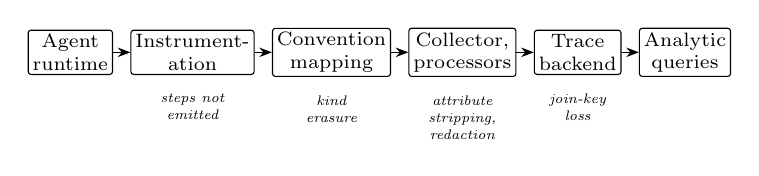
\begin{tikzpicture}[font=\scriptsize, node distance=2.2mm,
  box/.style={draw, rounded corners=1pt, minimum height=5.2mm, align=center, inner sep=1.6pt},
  arr/.style={-{Stealth[length=1.6mm]}}, loss/.style={align=center, font=\tiny\itshape}]
\node[box] (rt) {Agent\\runtime};
\node[box, right=of rt] (ins) {Instrument-\\ation};
\node[box, right=of ins] (conv) {Convention\\mapping};
\node[box, right=of conv] (col) {Collector,\\processors};
\node[box, right=of col] (be) {Trace\\backend};
\node[box, right=of be] (q) {Analytic\\queries};
\foreach \a/\b in {rt/ins, ins/conv, conv/col, col/be, be/q} \draw[arr] (\a) -- (\b);
\node[loss, below=1.2mm of ins] {steps not\\emitted};
\node[loss, below=1.2mm of conv] {kind\\erasure};
\node[loss, below=1.2mm of col] {attribute\\stripping,\\redaction};
\node[loss, below=1.2mm of be] {join-key\\loss};
\end{tikzpicture}}
\caption{Where structural information is lost between an agent runtime
and the queries run over its traces. The projection study models the
mapping and processing stages; E1 measures the instrumentation stage.}
\label{fig:pipeline}
\end{figure}

%% =====================================================================
\section{Methodology}
\label{sec:method}

\subsection{Projection study: data}

The projection study uses three corpora (Table~\ref{tab:corpora}): 112
SWE-bench~\cite{swebench} agent traces (3,060 events) and 56
end-to-end and multi-agent topology traces (626 events) from the
\textsc{AgentTelemetry} artifact~\cite{agenttelemetry_artifact}, and
1,980 historical $\tau$-bench~\cite{taubench} trajectories (42,581
derived events). The $\tau$-bench trajectories come with task outcomes
and expected tool-action labels. We convert them into sanitized event
traces that keep tool names, argument-shape counts, order and outcome,
but no messages, prompts, tool outputs or argument values.

\begin{table}[t]
\centering
\scriptsize
\caption{Corpora of the projection study.}
\label{tab:corpora}
\begin{tabular}{@{}p{0.15\columnwidth}rrp{0.50\columnwidth}@{}}
\toprule
Corpus & Traces & Events & Event kinds \\
\midrule
SWE-bench & 112 & 3,060 & agent, guardrail, LLM, memory, planning, reasoning, retrieval, tool \\
Topology & 56 & 626 & as above, plus delegation (109) \\
$\tau$-bench & 1,980 & 42,581 & agent, LLM (26,316), tool (14,285) \\
\bottomrule
\end{tabular}
\end{table}

\subsection{Projection study: schema views}

Table~\ref{tab:projections} defines seven views. The LLM-focused views
are mapped from OTel GenAI (main semantic-conventions repository,
commit f489c18), OpenInference (commit 0ee46c6) and OpenLLMetry
v0.61.0~\cite{otel_genai,openinference,openllmetry}. A field is retained
only when the cited convention exposes the corresponding span kind or
attribute family, and fields without a public anchor are counted absent.
Two choices drive results. First, the GenAI anchor was stale: by that
commit the GenAI conventions had moved to their own repository, which
already defined \texttt{invoke\_agent}, \texttt{plan} and memory
operations~\cite{otel_genai_repo}. The GenAI view therefore models
telemetry that carries only model, tool and retrieval operations, and we
label it \emph{GenAI model/tool}; it understates what the conventions
define. Second, the LLM+agent-run view keeps OpenInference's
\texttt{AGENT} and \texttt{GUARDRAIL} kinds. E1 tests both choices
against emitted telemetry. The
OTel+custom-attributes view stores the event kind as the attribute
\texttt{agent.event\_kind} rather than in a dedicated kind field.

\begin{table*}[t]
\centering
\scriptsize
\caption{Schema projections. Rows are field-family mappings, not
measurements of deployed products; E1 measures deployed instrumentation.}
\label{tab:projections}
\begin{tabular}{@{}p{0.13\textwidth}p{0.19\textwidth}p{0.33\textwidth}p{0.27\textwidth}@{}}
\toprule
Projection & Public anchor & Retained field families & Absent field families \\
\midrule
Vanilla OTel & OTel trace model & trace/span/parent IDs, timestamps, status & GenAI and agent diagnostic attributes \\
OTel+custom attrs & OTel span attributes & \texttt{agent.event\_kind} and non-content diagnostic attributes & dedicated event-kind field, payload content \\
GenAI model/tool & OTel GenAI spans & \texttt{gen\_ai.*} model/tool fields plus retrieval evidence & planning, reasoning, guardrail, delegation, memory, task labels \\
LLM+agent-run & OpenInference span kinds & \texttt{AGENT}, \texttt{LLM}, \texttt{TOOL}, \texttt{RETRIEVER}, \texttt{GUARDRAIL} & planning, reasoning loops, delegation, memory, tool-argument shape \\
LLM app & OpenLLMetry app traces & agent, LLM, tool, retrieval, token and tool-shape fields & planning, reasoning, guardrail, delegation, memory \\
Agent structural & agent structural extension & all event kinds plus structural and non-content diagnostic fields & prompt, completion, reasoning, retrieval and tool payload content \\
Agent reference & local reference schema & all sanitized fields & raw payload content \\
\bottomrule
\end{tabular}
\end{table*}

Each projection is replayed through the OpenTelemetry SDK into a SQLite
backend with separate span and attribute tables (740,272 span rows and
3,463,458 attribute rows across views and ablations, 1.18\,GiB), and
answerability is computed from backend rows. Per projection, export took
1.15--1.95\,s and three aggregate SQL queries 0.5--29.0\,ms, and attribute
rows ranged from 0 (vanilla) to 259,741 (reference). An OTel Collector
(otelcol-contrib 0.153.0) \texttt{otlpjsonfile}$\rightarrow$\texttt{file}
round trip of the custom-attribute view preserved all 46,267 spans,
258,617 diagnostic attributes and 44,119 parent links. Field ablations
remove one field class at a time from the reference view.

\subsection{E1: measuring emitted telemetry}
\label{sec:e1method}

\textbf{Agent.} A synthetic customer-support agent for an outdoor-gear
store handles 44 tickets. Each run reads customer memory, makes a
planning model call, retrieves policy excerpts, then iterates model
calls with seven tools. A deterministic guardrail checks every refund
(limit, window, order total) before it executes. Billing disputes are
delegated to a billing sub-agent with its own model loop and tools.
Tickets inject temporary tool failures, refunds that the guardrail
allows or blocks, billing disputes and stale remembered addresses
(Table~\ref{tab:tickets}). The
agent is implemented twice: as plain Python on the Anthropic SDK, and as
a LangGraph \texttt{StateGraph} with nodes for memory, planning,
retrieval, the model, the guardrail and tools, LangChain tools and
retriever, a LangGraph store, and a compiled billing subgraph. Model
calls use the Anthropic SDK in both, with model \texttt{claude-opus-5-5}
at effort \texttt{low}.

\begin{table}[t]
\centering
\scriptsize
\caption{E1 tickets. Each ticket runs once per implementation.}
\label{tab:tickets}
\begin{tabular}{@{}lrp{0.48\columnwidth}@{}}
\toprule
Category & Tickets & Injected condition \\
\midrule
Plain request & 5 & none \\
Temporary tool failure & 16 & order lookup fails 3--5 times; 8 tickets ask the agent to keep retrying \\
Refund allowed & 3 & within limit and window \\
Refund blocked & 7 & above limit or outside the 30-day window \\
Billing dispute & 8 & handled by delegation to the billing sub-agent \\
Stale memory & 3 & remembered address differs from the customer record \\
Combined & 2 & dispute with refund; failure with refund \\
\midrule
Total & 44 & \\
\bottomrule
\end{tabular}
\end{table}

\textbf{Same execution under every condition.} Each ticket runs live
once per implementation, and the HTTP exchanges with the API are
recorded at the transport layer. Each condition then replays the
recordings. Instrumentation wraps the SDK above the transport, so it
observes ordinary calls while plans, tool calls, failures and decisions
are identical across conditions. A replay that sends any request body
differing from the recording fails, and every replay must consume all
recorded exchanges. All 440 replays (88 executions, five conditions)
passed both checks. The 88 recorded executions made 441 model calls and
cost USD 2.96 including pilots.

\textbf{Conditions.} Each condition has its own environment with the
same base versions (anthropic 2.3.0, langgraph 1.2.17, langchain
1.4.7, OTel SDK 1.45.1) and default library settings: \emph{OpenInference}
(LangChain 0.1.80 and Anthropic 3.1.0 instrumentors); \emph{OpenLLMetry}
(LangChain and Anthropic instrumentors 0.62.4); \emph{OTel GenAI}, the
official LangChain and Anthropic instrumentations (1.3b0); and
\emph{AgentTelemetry}, an agent-aware reference that emits one span per
logical step. The Anthropic SDK emits its own metadata-only spans
whenever a tracer provider is registered, so its spans appear in every
condition, and an \emph{SDK-only} condition isolates them. Results
include the SDK spans, as a deployment would see them.

\textbf{Ground truth and scoring.} The agent logs every logical step
independently of OTel. Instances of the eight families are planning
steps, guardrail decisions, memory operations, delegations, tool
executions paired with the model call that requested them, model calls,
retrieval steps, and retry loops: three or more consecutive executions
of the same tool where every execution before the last failed. A span
matches an instance when their time intervals overlap. Each instance is
\emph{standard} if answerable from the library's documented attributes
plus generic structure (parent IDs, timestamps, status),
\emph{app-specific} if it also needs application naming such as
LangGraph node names, and otherwise \emph{not answerable}. Tool
provenance is standard only through a parent link or a tool-call ID
present on both spans; a link inferred from sibling order is
app-specific (Table~\ref{tab:mapping} lists the attributes accepted as
standard). The protocol was committed before any run. After the
first run, we added eight tickets asking the agent to keep retrying,
because it rarely retried three times in a row; the scoring rules did
not change.

\begin{table*}[t]
\centering
\scriptsize
\caption{Documented attributes accepted as standard when scoring E1. A
span's kind comes from the first kind attribute present; identity,
token and call-ID keys are accepted from any library.}
\label{tab:mapping}
\setlength{\tabcolsep}{4pt}
\begin{tabular}{@{}>{\raggedright\arraybackslash}p{0.11\textwidth}>{\raggedright\arraybackslash}p{0.27\textwidth}>{\raggedright\arraybackslash}p{0.25\textwidth}>{\raggedright\arraybackslash}p{0.13\textwidth}>{\raggedright\arraybackslash}p{0.15\textwidth}@{}}
\toprule
Source & Kind & Tool and agent identity & Tokens & Tool-call ID \\
\midrule
OpenInference & \texttt{openinference.span.kind} (LLM, TOOL, RETRIEVER, AGENT, CHAIN, GUARDRAIL) & \texttt{tool.name}; \texttt{agent.name} & \texttt{llm.token\_count.*} & \texttt{tool\_call.id} \\
OpenLLMetry & \texttt{gen\_ai.operation.name}, else \texttt{traceloop.span.kind} (workflow, task, agent, tool) & \texttt{gen\_ai.tool.name}, \texttt{traceloop.entity.name} on tool spans; \texttt{gen\_ai.agent.name} & \texttt{gen\_ai.usage.*} & \texttt{gen\_ai.tool.call.id} \\
OTel GenAI, SDK & \texttt{gen\_ai.operation.name} (chat, execute\_tool, retrieval, invoke\_agent, invoke\_workflow) & \texttt{gen\_ai.tool.name}; \texttt{gen\_ai.agent.name} & \texttt{gen\_ai.usage.*} & \texttt{gen\_ai.tool.call.id} \\
AgentTelemetry & \texttt{agenttelemetry.span.kind} (nine agent kinds) & \texttt{tool.name}; \texttt{agent.name}, \texttt{delegation.target\_agent} & \texttt{llm.*\_tokens} & \texttt{tool.call\_id} \\
\bottomrule
\end{tabular}
\end{table*}

\subsection{Reproducibility}

E1's code, recorded API exchanges, spans, ground truth and scores are
provided as anonymized supplementary material. Replaying the recordings
requires no API key. The projection-study numbers are reported from the
original analysis of the public \textsc{AgentTelemetry} and
$\tau$-bench data.

%% =====================================================================
\section{Results}
\label{sec:results}

\subsection{RQ1: Projections preserve partial answerability}
\label{sec:rq1}

\begin{table}[t]
\centering
\scriptsize
\caption{Projection metrics over the pooled backend. Kinds counts a
dedicated kind field. Macro Q weights each query family equally; Inst.\
Q pools instances and is dominated by token accounting.}
\label{tab:interop}
\begin{tabular}{@{}lrrrr@{}}
\toprule
Projection & Kinds & Attrs & Macro Q & Inst. Q \\
\midrule
Vanilla OTel & 0.0\% & 0.0\% & 0.0\% & 0.00\% \\
OTel+custom attrs & 0.0\% & 100.0\% & 100.0\% & 100.00\% \\
GenAI model/tool & 33.3\% & 31.6\% & 37.5\% & 99.97\% \\
LLM+agent-run & 55.6\% & 47.4\% & 50.0\% & 99.97\% \\
LLM app & 44.4\% & 47.4\% & 37.5\% & 99.97\% \\
Agent structural & 100.0\% & 100.0\% & 100.0\% & 100.00\% \\
Agent reference & 100.0\% & 100.0\% & 100.0\% & 100.00\% \\
\bottomrule
\end{tabular}
\end{table}

\begin{figure}[t]
\centering
\resizebox{\columnwidth}{!}{%
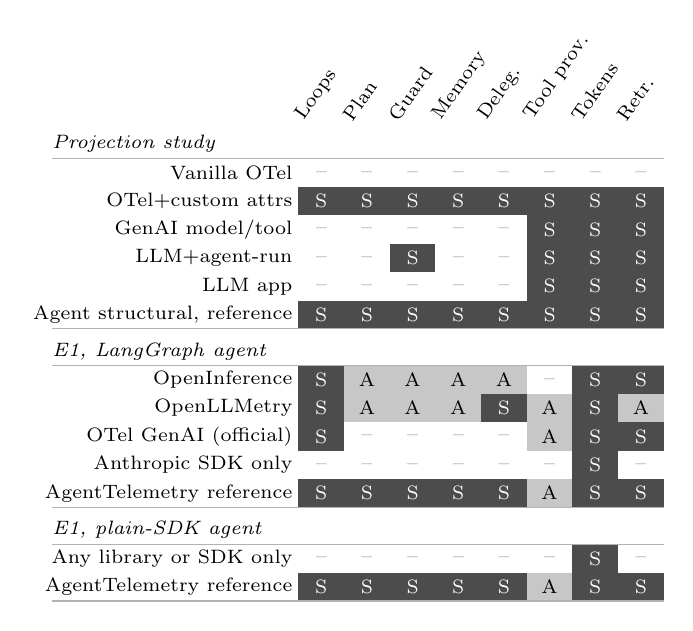
\begin{tikzpicture}[font=\scriptsize, x=5.8mm, y=-3.6mm]
\def\SSS{S}\def\AAA{A}\def\NNN{N}
\foreach \f [count=\i from 0] in {Loops,Plan,Guard,Memory,Deleg.,Tool prov.,Tokens,Retr.}
  \node[rotate=55, anchor=south west, inner sep=1pt] at (\i+0.2,-0.1) {\f};
\newcommand{\drawrow}[3]{%
  \node[anchor=east, inner sep=2pt] at (0,#1+0.5) {#2};
  \foreach \c [count=\j from 0] in {#3} {%
    \ifx\c\SSS \fill[black!70] (\j,#1) rectangle (\j+1,#1+1); \node[white] at (\j+0.5,#1+0.5) {S};\fi
    \ifx\c\AAA \fill[black!22] (\j,#1) rectangle (\j+1,#1+1); \node at (\j+0.5,#1+0.5) {A};\fi
    \ifx\c\NNN \node[black!45] at (\j+0.5,#1+0.5) {--};\fi}}
\newcommand{\group}[2]{\node[anchor=west, font=\scriptsize\itshape, inner sep=0pt] at (-5.4,#1+0.5) {#2};}
\group{-0.05}{Projection study}
\drawrow{1}{Vanilla OTel}{N,N,N,N,N,N,N,N}
\drawrow{2}{OTel+custom attrs}{S,S,S,S,S,S,S,S}
\drawrow{3}{GenAI model/tool}{N,N,N,N,N,S,S,S}
\drawrow{4}{LLM+agent-run}{N,N,S,N,N,S,S,S}
\drawrow{5}{LLM app}{N,N,N,N,N,S,S,S}
\drawrow{6}{Agent structural, reference}{S,S,S,S,S,S,S,S}
\group{7.3}{E1, LangGraph agent}
\drawrow{8.3}{OpenInference}{S,A,A,A,A,N,S,S}
\drawrow{9.3}{OpenLLMetry}{S,A,A,A,S,A,S,A}
\drawrow{10.3}{OTel GenAI (official)}{S,N,N,N,N,A,S,S}
\drawrow{11.3}{Anthropic SDK only}{N,N,N,N,N,N,S,N}
\drawrow{12.3}{AgentTelemetry reference}{S,S,S,S,S,A,S,S}
\group{13.6}{E1, plain-SDK agent}
\drawrow{14.6}{Any library or SDK only}{N,N,N,N,N,N,S,N}
\drawrow{15.6}{AgentTelemetry reference}{S,S,S,S,S,A,S,S}
\foreach \y in {1,7,8.3,13.3,14.6,16.6} \draw[black!30] (-5.4,\y) -- (8,\y);
\end{tikzpicture}}
\caption{Projected versus measured answerability. Top: projection study
(answerable or not, by construction). Middle and bottom: E1, where every
instance in a family received the same level: S = standard attributes,
A = only with application-specific names or sibling order, -- = not
answerable. ``Any library'' covers OpenInference, OpenLLMetry and OTel
GenAI. E1's Loops family counts tool retry loops. Instances per
framework (plain/LangGraph): Loops 7/10, Plan 44/44, Guard 9/9, Memory
88/88, Deleg.\ 13/11, Tool prov.\ 165/161, Tokens 223/218, Retr.\ 63/63.}
\label{fig:heatmap}
\end{figure}

Table~\ref{tab:interop} and the top of Fig.~\ref{fig:heatmap} report the
projection study. The LLM-focused views keep 33.3--55.6\% of event kinds
and answer 37.5--50.0\% of the families. They answer the tool, token and
retrieval families, and none of planning, loops, memory or delegation;
the OpenInference-anchored view also answers guardrail audits. These
outcomes follow from the projection rules in Table~\ref{tab:projections}
and the requirements in Table~\ref{tab:queries}. That is the point of a
specification-level analysis: it states precisely which questions a
schema can and cannot answer. Whether deployed instrumentation behaves
this way is the subject of RQ3. The OTel+custom-attributes view shows
the opposite case. It scores 0\% on dedicated kinds but answers every
family, because the kind survives as an attribute. Generic span storage
therefore does not destroy agent semantics as long as the fields survive
somewhere. Recall against the reference is 100\% for the reference and
structural views by definition, because reference counts are computed on
the reference view (instances: loops 113, planning 162, guardrail 80,
memory 257, delegation 109, tool provenance 14,427, token records
2,167,286, retrieval 685).

The choice of metric matters. Pooling instances (Inst.\ Q) gives the
LLM-focused views 99.97\%, because token accounting contributes
2,167,286 of 2,183,119 positive instances. Macro Q exposes the
orchestration gap that pooling hides. By corpus, the tool-heavy
$\tau$-bench workload loses little (both of its applicable families are
answered), while the SWE-bench and topology corpora drop to
37.5--42.9\% under the LLM-focused views.

On $\tau$-bench we also tested whether missing expected actions predict
task failure. They do not: the proxy reaches 57.9\% F1 against 57.4\%
for always predicting failure, and it gives the same result for every
view that keeps tool calls, so it does not discriminate between schemas.
The expected actions that are not visible (33.8\%) are actions the agent
never took. That is agent behavior, not schema loss, and we no longer
treat this proxy as evidence about schemas.

\subsection{RQ2: Field classes are individually load-bearing}

\begin{table*}[t]
\centering
\scriptsize
\caption{Field ablations on the reference view. Each row removes one
field class and keeps the rest of the backend intact.}
\label{tab:ablation}
\begin{tabular}{@{}lrrrrp{0.40\textwidth}@{}}
\toprule
Ablation & Kinds & Attrs & Joins & Query recall & Failed families \\
\midrule
Drop semantic kind & 0.0\% & 94.7\% & 100.0\% & 0.0\% & all eight \\
Collapse orchestration kinds & 44.4\% & 94.7\% & 100.0\% & 37.5\% & loops, planning, guardrail, memory, delegation \\
Drop parent IDs & 100.0\% & 100.0\% & 0.0\% & 87.5\% & tool provenance \\
Drop timestamps & 100.0\% & 100.0\% & 100.0\% & 87.5\% & loops \\
Drop agent IDs & 100.0\% & 89.5\% & 100.0\% & 100.0\% & none \\
Drop memory attrs & 100.0\% & 89.5\% & 100.0\% & 87.5\% & memory \\
Drop guardrail attrs & 100.0\% & 94.7\% & 100.0\% & 87.5\% & guardrail \\
Drop token/cost & 100.0\% & 89.5\% & 100.0\% & 87.5\% & tokens \\
Content redaction & 100.0\% & 100.0\% & 100.0\% & 100.0\% & none \\
\bottomrule
\end{tabular}
\end{table*}

Table~\ref{tab:ablation} separates design mistakes that a coarse
projection hides. Dropping the event kind (both the dedicated field and
the custom attribute) makes every family unanswerable even though most
attributes remain. Collapsing only the orchestration kinds reproduces
the 37.5\% of the LLM-focused views. Dropping parent identifiers keeps
kinds and attributes but breaks tool provenance, dropping timestamps
breaks loop detection, which is an ordered phenomenon, and dropping
memory, guardrail or token attributes breaks the matching family.
Content redaction preserves all eight families: they need kinds, order,
join keys and selected non-content attributes, not prompts,
completions, reasoning text, tool payloads or retrieved content.
Payload remains necessary for other tasks, such as judging whether a
document grounded an answer or whether an argument value was correct.

\subsection{RQ3: What instrumentation actually emits}

\begin{table}[t]
\centering
\scriptsize
\caption{E1 trace structure per agent execution (means over 44 runs,
SDK spans included). Agent spans counts spans labelled as an agent;
in parentheses, those whose identity is neither of the two real
agents. Content: prompts or responses captured by default.}
\label{tab:e1structure}
\setlength{\tabcolsep}{3.2pt}
\begin{tabular}{@{}lrrrrrc@{}}
\toprule
& \multicolumn{2}{c}{Plain SDK} & \multicolumn{3}{c}{LangGraph} & \\
\cmidrule(lr){2-3}\cmidrule(lr){4-6}
Condition & Spans & Traces & Spans & Traces & Agent spans & Content \\
\midrule
SDK only & 5.1 & 5.07 & 5.0 & 4.95 & 0.0 (0.0) & no \\
OpenInference & 10.1 & 5.07 & 31.1 & 5.95 & 8.3 (7.3) & yes \\
OpenLLMetry & 10.1 & 10.14 & 32.3 & 1.00 & 2.3 (0.0) & yes \\
OTel GenAI & 10.1 & 5.07 & 19.3 & 1.00 & 4.3 (3.3) & no \\
AgentTelemetry & 24.2 & 1.00 & 23.7 & 1.00 & 1.3 (0.0) & no \\
\bottomrule
\end{tabular}
\end{table}

The lower part of Fig.~\ref{fig:heatmap} and Table~\ref{tab:e1structure}
report E1. Every instance within a family received the same level, so
each cell is 100\% of its instances. The uncertainty therefore lies in
how far other agents behave alike, not in these estimates: a 95\%
Wilson interval for a full cell has a lower bound of 64.6\% for the
smallest family (7 loops) and 92.0\% for 44 planning steps. Six
findings stand out.

\textbf{Without a framework, schemas do not matter.} For the plain-SDK
agent, all three libraries and the SDK emit only model-call spans. Token
accounting is fully answerable and nothing else is: planning, retrieval,
tools, guardrails, memory and delegation happen in application code
that no instrumentation sees. The calls are not even connected. Each
model call starts its own trace (5.07 traces per execution), and under
OpenLLMetry the library span and the SDK span of the same call land in
separate traces (10.14).

\textbf{With LangGraph, orchestration becomes visible, but not as
semantics.} Node spans make planning, memory and guardrail steps
recoverable under OpenInference and OpenLLMetry, but only by node name
(\texttt{planner}, \texttt{load\_memory}, \texttt{refund\_guardrail}).
No library identified them through a standard construct, although
the GenAI conventions define \texttt{plan} and memory operations and
OpenInference defines \texttt{GUARDRAIL}. The guardrail decision
appears only inside captured node output. The official OTel GenAI
instrumentation omits these nodes entirely. This confirms the
projection study's central prediction for planning, memory and
guardrails, and it refutes the LLM+agent-run view's assumption that
guardrails arrive as a standard kind.

\textbf{Retry loops and failures are visible from tool spans.} With
LangGraph, every library marks failed tool executions with error status
(50 of 50 failures) and preserves order, so all ten retry loops are
standard-answerable. The projections predicted 0\% for loops in the
LLM-focused views, because they modeled loops through reasoning kinds;
retry loops in particular need only tool spans.

\textbf{No library links a tool to its decision.} OpenInference emits
its model-call spans outside the LangGraph trace (5.95 traces per
execution), so its tool spans cannot be related to model calls at all.
OpenLLMetry and OTel GenAI keep one trace, but tools and model calls
are siblings under different nodes, so provenance can only be inferred
from order. OTel GenAI records \texttt{gen\_ai.tool.call.id} on tool
spans, but the matching ID on the model-call side exists only inside
message content, which it does not capture by default. Explicit
provenance therefore requires capturing content, which pulls against
payload redaction. The projections assumed tool provenance in every
LLM-focused view; measured, it is standard in none.

\textbf{Agent identity is inconsistent.} Only OpenLLMetry emits an
\texttt{invoke\_agent} span for the delegated billing sub-agent (11 of
11 delegations). OTel GenAI emits none for it and attributes the
sub-agent's tool calls to the parent \texttt{support\_agent} (16 of 16
billing tool spans). Both OpenInference and OTel GenAI label the router
function \texttt{route\_after\_agent} as an agent. OpenInference marks
every run whose name contains ``agent'' as \texttt{AGENT}, so the nodes
\texttt{agent} and \texttt{billing\_agent} become agents while the
billing subgraph itself is a \texttt{CHAIN}.
Queries that count or group by agent therefore return wrong answers
under these libraries (Table~\ref{tab:e1structure}, Fig.~\ref{fig:delegation}).

\begin{figure*}[t]
\centering
\newcommand{\tl}[2]{\par\noindent\hspace*{#1em}{\tiny\texttt{#2}}}
\newcommand{\nt}[2]{\par\noindent\hspace*{#1em}{\tiny\emph{#2}}}
\begin{minipage}[t]{0.24\textwidth}
\footnotesize\textbf{OpenInference}
\tl{0}{escalate\_to\_billing [TOOL]}
\tl{1}{billing\_specialist [CHAIN]}
\tl{2}{billing\_agent [AGENT] x3}
\tl{2}{route [CHAIN] x3}
\tl{2}{billing\_tools [CHAIN] x2}
\tl{3}{lookup\_invoice [TOOL]}
\tl{3}{apply\_credit [TOOL]}
\tl{0}{messages.create [LLM] x3}
\nt{1}{each in its own trace}
\end{minipage}\hfill
\begin{minipage}[t]{0.24\textwidth}
\footnotesize\textbf{OpenLLMetry}
\tl{0}{escalate\_to\_billing [tool]}
\tl{1}{billing\_specialist [invoke\_agent]}
\tl{1}{billing\_specialist [task]}
\tl{2}{billing\_agent [task] x3}
\tl{3}{anthropic.chat [chat]}
\tl{2}{billing\_tools [task] x2}
\tl{3}{lookup\_invoice [tool]}
\tl{3}{apply\_credit [tool]}
\end{minipage}\hfill
\begin{minipage}[t]{0.24\textwidth}
\footnotesize\textbf{OTel GenAI (official)}
\tl{0}{escalate\_to\_billing [execute\_tool]}
\nt{1}{agent: support\_agent}
\tl{1}{chat claude-opus-5-5 x3}
\tl{1}{lookup\_invoice [execute\_tool]}
\nt{2}{agent: support\_agent}
\tl{1}{apply\_credit [execute\_tool]}
\nt{2}{agent: support\_agent}
\nt{0}{no span for billing\_specialist}
\end{minipage}\hfill
\begin{minipage}[t]{0.24\textwidth}
\footnotesize\textbf{AgentTelemetry reference}
\tl{0}{escalate\_to\_billing [TOOL\_CALL]}
\tl{1}{delegate\_to\_billing [DELEGATION]}
\tl{2}{billing\_specialist [AGENT]}
\tl{3}{billing\_iteration [REASONING] x3}
\tl{4}{model\_call [LLM\_CALL]}
\tl{3}{lookup\_invoice [TOOL\_CALL]}
\tl{3}{apply\_credit [TOOL\_CALL]}
\end{minipage}
\caption{One recorded delegation (ticket S16, LangGraph agent) as stored by
each condition, indented by parent, with the span kind or operation in
brackets; OpenLLMetry's name prefixes and SDK spans are omitted. The execution is
identical in all four. Only OpenLLMetry and the reference name the billing
sub-agent with a standard agent construct, and in OpenLLMetry the sub-agent's
steps are siblings of its \texttt{invoke\_agent} span rather than its
children. OTel GenAI attributes the sub-agent's tools to the parent agent.}
\label{fig:delegation}
\end{figure*}

\textbf{Defaults decide what is stored.} OpenInference and OpenLLMetry
capture prompts and responses by default; OTel GenAI and the SDK record
metadata only. The official LangChain instrumentation also requires the
\texttt{langchain} package: with only \texttt{langchain-core}, as in a
LangGraph-only application, it logs an error and emits nothing, so the
framework spans silently disappear.

E1's backend held 7,524 spans and 122,998 attribute rows (32\,MiB).
Per execution, the libraries produced 215--628 attribute rows with
LangGraph, against 207 for the agent-aware reference, so the reference
answers more families with fewer rows.

%% =====================================================================
\section{Discussion}
\label{sec:discussion}

\textbf{Agent observability is a data pipeline.} The quality of an
agent trace store is decided at every stage of
Fig.~\ref{fig:pipeline}. E1 shows that the instrumentation stage alone
can decide most of it: the same execution yields a store that answers
one family or seven, depending on framework and library, before any
collector or backend is involved. Evaluations of observability stacks
should therefore include downstream queries scored against ground
truth, not only export success or ingestion throughput.

\textbf{Projections need validation against emitted telemetry.} The
projection study was right about the absence of standard planning,
memory and guardrail semantics, and wrong in both directions elsewhere:
too optimistic about tool provenance and guardrail kinds, too
pessimistic about retry loops and, for OpenLLMetry, delegation. A
schema that defines a construct does not guarantee that instrumentation
emits it.

\begin{table}[t]
\centering
\scriptsize
\caption{Defined in a convention versus emitted with standard attributes
in E1 (LangGraph agent, default settings).}
\label{tab:defined}
\begin{tabular}{@{}lp{0.38\columnwidth}p{0.33\columnwidth}@{}}
\toprule
Family & Defined construct & Emitted standardly by \\
\midrule
Loops & no loop construct; tool spans with status suffice for retries & all three libraries \\
Plan & OTel \texttt{plan} & none \\
Guard & OpenInference \texttt{GUARDRAIL} & none \\
Memory & OTel memory operations & none \\
Deleg. & OTel \texttt{invoke\_agent}; OpenInference \texttt{AGENT} & OpenLLMetry only \\
Tool prov. & \texttt{gen\_ai.tool.call.id} (model side only in content) & none (order only) \\
Tokens & usage attributes in all three & all three and the SDK \\
Retr. & OTel \texttt{retrieval}; OpenInference \texttt{RETRIEVER} & OpenInference, OTel GenAI \\
\bottomrule
\end{tabular}
\end{table}

\textbf{Defined is not emitted.} Table~\ref{tab:defined} summarizes the
gap. For four of the eight families a convention already defines the
needed construct, yet no library emits it for a LangGraph agent. The
bottleneck for agent trace quality is thus less the vocabulary than the
mapping from framework steps onto it.

\textbf{Implications for conventions and instrumentation.} (1) Planning
and memory operations are defined in the GenAI conventions but not
emitted, and guardrails have no operation; instrumentation needs to map
framework steps onto these constructs, because application node names
are not portable across services or teams.
(2) The tool-call ID should be a structured attribute on both the tool
span and the model-call span, outside message content, so provenance
survives payload redaction. (3) Agent identification should rest on
explicit declarations, not on name heuristics that turn routers into
agents, and nested agents invoked from tools need their own invocation
spans. (4) An instrumentation library that cannot activate should fail
loudly. (5) Pipelines should record which semantic fields were
intentionally unavailable, so analytics can refuse questions rather
than answer them from incomplete data.

\textbf{Answerability tests as data-quality checks.} E1's harness doubles
as a regression test for telemetry pipelines. Record representative
agent executions once, replay them through the instrumentation and
collector configuration under test, and assert the query families an
organization relies on against ground truth, much as data-validation
systems unit-test datasets before they are consumed~\cite{deequ}. Unlike
checks of export success, such tests catch instrumentation that silently
does nothing, renamed nodes that break application mappings, library
upgrades that change span kinds, and processors that strip fields.
Replay needs no model access, so the tests are cheap and deterministic.

\textbf{Privacy.} The payload-redaction result and E1's defaults point
the same way. Structural fields carry most diagnostic value, while two
of three libraries store content by default. A metadata-first default
with structural agent fields, as OTel GenAI and the SDK already do for
content, would give analysts more structure with less sensitive data.
Structural fields still reveal workflow shape and need ordinary access
control and retention policies.

%% =====================================================================
\section{Threats to Validity}
\label{sec:threats}

\textbf{Projections are analytical.} Their answerability follows from
mapping rules. We report them as a specification-level analysis and
test them with E1 rather than presenting them as measurements of
products.

\textbf{E1 covers one agent, one domain and one model.} The agent is
synthetic and small, its tickets were written by the authors, and the
model is fixed. The two implementations bracket common practice
(framework-free code and LangGraph) but not frameworks with their own
agent abstractions, such as CrewAI or the OpenAI Agents SDK, which may
fare better. Default settings were kept on purpose; libraries offer
hooks, such as metadata hints or custom attributes, that could raise
answerability at engineering cost. Library versions change quickly, so
results are pinned to the versions listed.

\textbf{Scoring choices.} The app-specific level depends on the names
we chose for nodes; a team with different conventions needs a different
mapping, which is exactly why we do not count it as standard. Time
overlap matching could over-match nested spans; family predicates
require the matching kind or name, which limits this. Guardrail (9 per
implementation) and loop (7 and 10) instances are few, though every
instance received the same level.

\textbf{Scale.} The backends are SQLite stores of 0.7\,M (projection)
and 7.5\,k (E1) spans, not Jaeger, Tempo, ClickHouse or OpenSearch at
production volume. The study is about which semantics reach a store,
which does not depend on volume, but cost and query behavior at scale
are not measured. The projection traces and fault definitions come from
one prior artifact, and E1 adds an independent, orchestration-heavy
workload.

%% =====================================================================
\section{Related Work}
\label{sec:related}

\textbf{Tracing and trace data.} Dapper, X-Trace and Magpie established
structured request tracing~\cite{dapper,xtrace,magpie}, and Canopy
showed how trace data must be transformed into analysis-ready datasets
at scale~\cite{canopy}. Sifter and Hindsight decide which traces to
keep~\cite{sifter,hindsight}, a question of data volume; we study which
fields survive within the traces that are kept. Loghub made system logs
an analyzable data asset~\cite{loghub}; agent traces call for similar
attention to the fields analytics need.

\textbf{Data quality, schemas and provenance.} Data quality is fitness
for consumer tasks~\cite{wang_strong,batini}. Schema
matching~\cite{rahm_bernstein} and schema evolution~\cite{prism} study
how mappings and versions change what data can express, and provenance
explains how answers depend on what survives a
pipeline~\cite{cheney_provenance}. We apply these lenses to span stores
fed by evolving conventions.

\textbf{LLM and agent observability.} OTel GenAI, OpenInference,
OpenLLMetry, LangSmith and Langfuse define and implement LLM
tracing~\cite{otel_genai,otel_agent_spans,openinference,openllmetry,langsmith,langfuse}.
Failure taxonomies and debugging tools for agents motivate the families
we
measure~\cite{mast,agentops,agdebugger,agenttelemetry_aiware}, and
$\tau$-bench supplies tool-agent workloads with outcomes~\cite{taubench}.
To our knowledge, prior work has not compared, instance by instance,
what different instrumentation libraries emit for identical agent
executions.

%% =====================================================================
\section{Conclusion}
\label{sec:conclusion}

Agent traces can be complete in rows and incomplete in meaning. The
projection study shows which fields each structural query needs, that
LLM-focused schemas answer 37.5--50.0\% of the query families, and that
payload can be redacted without losing structure. E1 shows what
deployed instrumentation actually stores. Without a framework, only
model calls. With LangGraph, loops, tools and retrieval, but planning,
memory and guardrails only under application names, no standard tool
provenance, and inconsistent agent identity. Agent observability needs
schema contracts that are checked against emitted telemetry, not only
written down.

\section*{AI Usage Disclosure}
Generative AI (Anthropic Claude, used through Claude Code) was used
substantively for this paper: to rebuild the LaTeX source, design and
implement the E1 harness and scoring code, run the experiments, analyze
results, produce figures and tables, and draft and edit text. In E1,
Claude Opus 5.5 is also the model inside the studied agent. The authors
reviewed and verified all code, data, results and text, and take full
responsibility for them.

%% =====================================================================
\balance
\begin{thebibliography}{10}
\providecommand{\url}[1]{#1}
\csname url@samestyle\endcsname
\providecommand{\newblock}{\relax}
\providecommand{\bibinfo}[2]{#2}
\providecommand{\BIBentrySTDinterwordspacing}{\spaceskip=0pt\relax}
\providecommand{\BIBentryALTinterwordstretchfactor}{4}
\providecommand{\BIBentryALTinterwordspacing}{\spaceskip=\fontdimen2\font plus
\BIBentryALTinterwordstretchfactor\fontdimen3\font minus
  \fontdimen4\font\relax}
\providecommand{\BIBdecl}{\relax}
\BIBdecl

\bibitem{wang_strong}
R.~Y. Wang and D.~M. Strong, ``Beyond accuracy: What data quality means to data
  consumers,'' \emph{Journal of Management Information Systems}, vol.~12,
  no.~4, pp. 5--33, 1996.

\bibitem{batini}
C.~Batini, C.~Cappiello, C.~Francalanci, and A.~Maurino, ``Methodologies for
  data quality assessment and improvement,'' \emph{ACM Computing Surveys},
  vol.~41, no.~3, pp. 1--52, 2009.

\bibitem{otel_spec}
\BIBentryALTinterwordspacing
{OpenTelemetry Authors}, ``{OpenTelemetry Specification},'' 2024. [Online].
  Available: \url{https://opentelemetry.io/docs/specs/otel/}
\BIBentrySTDinterwordspacing

\bibitem{otel_genai}
------, ``{OpenTelemetry} semantic conventions for {GenAI} operations,''
  \url{https://opentelemetry.io/docs/specs/semconv/gen-ai/}, 2026.

\bibitem{otel_agent_spans}
------, ``Semantic conventions for {GenAI} agent and framework spans,''
  \url{https://opentelemetry.io/docs/specs/semconv/gen-ai/gen-ai-agent-spans/},
  2026.

\bibitem{otel_genai_repo}
------, ``Semantic conventions for generative {AI},''
  \url{https://github.com/open-telemetry/semantic-conventions-genai}, commit
  0b9555d, Oct. 2026.

\bibitem{openinference}
\BIBentryALTinterwordspacing
{Arize AI}, ``{OpenInference}: Semantic conventions for {LLM}, {ML}, and agent
  observability,'' 2026. [Online]. Available:
  \url{https://github.com/Arize-ai/openinference}
\BIBentrySTDinterwordspacing

\bibitem{openllmetry}
{Traceloop}, ``{OpenLLMetry}: Open-source observability for {LLM}
  applications,'' \url{https://github.com/traceloop/openllmetry}, 2026.

\bibitem{dapper}
\BIBentryALTinterwordspacing
B.~H. Sigelman, L.~A. Barroso, M.~Burrows, P.~Stephenson, M.~Plakal, D.~Beaver,
  S.~Jaspan, and C.~Shanbhag, ``{Dapper, a Large-Scale Distributed Systems
  Tracing Infrastructure},'' Google, Tech. Rep. dapper-2010-1, 2010.
\BIBentrySTDinterwordspacing

\bibitem{xtrace}
R.~Fonseca, G.~Porter, R.~H. Katz, S.~Shenker, and I.~Stoica, ``{X-Trace}: A
  pervasive network tracing framework,'' in \emph{Proc. 4th USENIX Symposium on
  Networked Systems Design and Implementation (NSDI)}, 2007.

\bibitem{magpie}
P.~Barham, A.~Donnelly, R.~Isaacs, and R.~Mortier, ``Using {Magpie} for request
  extraction and workload modelling,'' in \emph{Proc. 6th Symposium on Operating
  Systems Design and Implementation (OSDI)}, 2004.

\bibitem{mast}
M.~Cemri, M.~Z. Pan, S.~Yang, L.~A. Agrawal, B.~Chopra, R.~Tiwari, K.~Keutzer,
  A.~Parameswaran, D.~Klein, K.~Ramchandran, M.~Zaharia, J.~E. Gonzalez, and
  I.~Stoica, ``Why do multi-agent {LLM} systems fail?'' \emph{arXiv preprint
  arXiv:2503.13657}, 2025.

\bibitem{agentops}
L.~Dong, Q.~Lu, and L.~Zhu, ``{AgentOps}: Enabling observability of {LLM}
  agents,'' 2024.

\bibitem{agdebugger}
W.~Epperson, G.~Bansal, V.~Dibia, A.~Fourney, J.~Gerrits, E.~Zhu, and
  S.~Amershi, ``Interactive debugging and steering of multi-agent {AI}
  systems,'' in \emph{Proc. 2025 CHI Conference on Human Factors in Computing
  Systems}, 2025.

\bibitem{agenttelemetry_aiware}
K.~C. Balusu, ``{AgentTelemetry}: A fault detection benchmark and toolkit for
  {LLM} agent observability,'' in \emph{Proc. 3rd ACM International Conference
  on AI-Powered Software (AIware '26)}, 2026.

\bibitem{agenttelemetry_artifact}
------, ``{AgentTelemetry}: Reproduction artifact,'' 2026.

\bibitem{swebench}
C.~E. Jimenez, J.~Yang, A.~Wettig, S.~Yao, K.~Pei, O.~Press, and K.~Narasimhan,
  ``{SWE-bench}: Can language models resolve real-world {GitHub} issues?'' in
  \emph{Proc. 12th International Conference on Learning Representations
  (ICLR)}, 2024.

\bibitem{taubench}
S.~Yao, N.~Shinn, P.~Razavi, and K.~Narasimhan, ``$\tau$-bench: A benchmark for
  tool-agent-user interaction in real-world domains,'' \emph{arXiv preprint
  arXiv:2406.12045}, 2024.

\bibitem{canopy}
J.~Kaldor \emph{et~al.}, ``Canopy: An end-to-end performance tracing and
  analysis system,'' in \emph{Proc. 26th ACM Symposium on Operating Systems
  Principles (SOSP)}, 2017, pp. 34--50.

\bibitem{sifter}
P.~Las-Casas, G.~Papakerashvili, V.~Anand, and J.~Mace, ``Sifter: Scalable
  sampling for distributed traces, without feature engineering,'' in
  \emph{Proc. ACM Symposium on Cloud Computing (SoCC)}, 2019.

\bibitem{hindsight}
L.~Zhang, Z.~Xie, V.~Anand, Y.~Vigfusson, and J.~Mace, ``The benefit of
  hindsight: Tracing edge-cases in distributed systems,'' in \emph{Proc. 20th
  USENIX Symposium on Networked Systems Design and Implementation (NSDI)},
  2023, pp. 321--339.

\bibitem{loghub}
J.~Zhu, S.~He, P.~He, J.~Liu, and M.~R. Lyu, ``Loghub: A large collection of
  system log datasets for {AI}-driven log analytics,'' in \emph{Proc. 34th
  IEEE International Symposium on Software Reliability Engineering (ISSRE)},
  2023.

\bibitem{rahm_bernstein}
E.~Rahm and P.~A. Bernstein, ``A survey of approaches to automatic schema
  matching,'' \emph{The VLDB Journal}, vol.~10, no.~4, pp. 334--350, 2001.

\bibitem{prism}
C.~Curino, H.~J. Moon, and C.~Zaniolo, ``Graceful database schema evolution:
  The {PRISM} workbench,'' \emph{Proc. VLDB Endowment}, vol.~1, no.~1, 2008.

\bibitem{cheney_provenance}
J.~Cheney, L.~Chiticariu, and W.-C. Tan, ``Provenance in databases: Why, how,
  and where,'' \emph{Foundations and Trends in Databases}, vol.~1, no.~4, pp.
  379--474, 2009.

\bibitem{deequ}
S.~Schelter \emph{et~al.}, ``Automating large-scale data quality
  verification,'' \emph{Proc. VLDB Endowment}, vol.~11, no.~12, pp.
  1781--1794, 2018.

\bibitem{langsmith}
{LangChain, Inc.}, ``{LangSmith}: Platform for {LLM} application development,
  monitoring, and testing,'' \url{https://smith.langchain.com}, 2026.

\bibitem{langfuse}
{Langfuse}, ``{Langfuse}: Open-source {LLM} engineering platform,''
  \url{https://github.com/langfuse/langfuse}, 2026.

\end{thebibliography}

\end{document}
